 
\chapter{Выбор рациональной конструкции}
Как было отмечено в разделе \ref{sec:ndsResults}, одним из проблемных с точки зрения прочности мест конструкции гипотетического БПЛА является элемент конструкции, обеспечивающий основное крепление хвостовой части к центропланом. В целях нахождения конструкции гипотетического БПЛА минимального веса в работе был проведен сравнительный анализ различных вариантов исполнения данного элемента. Для проведения анализа были выбраны три варианта конструкции, представленные на схемах на Рис.\ref{fig:variants_plain} и изображениях МКЭ-моделей на Рис.\ref{fig:variants_mke}. Для анализа была использована модель, описанная в разделе \ref{sec:creationOfOneModel} и две модели, созданные на её основе. Все три модели были адаптированы с учетом выводов, которые будут получены в разделе \ref{sec:optimalMKESize}.  

\begin{figure}[H]
\centering
\captionsetup{justification=centering}
\begin{subfigure}[b]{0.32\textwidth}
\centering
	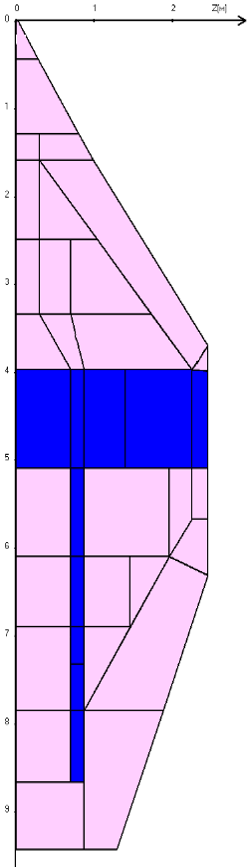
\includegraphics[width=0.3\textwidth]{variants/1_plain}
	\caption{Вариант 1}
\end{subfigure}
\hspace{\fill}
\begin{subfigure}[b]{0.32\textwidth}
\centering
	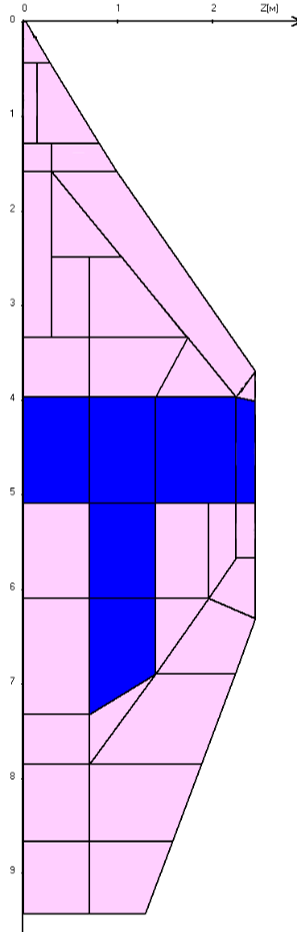
\includegraphics[width=0.3\textwidth]{variants/2_plain}
	\caption{Вариант 2}
\end{subfigure}
\hspace{\fill}
\begin{subfigure}[b]{0.32\textwidth}
\centering
	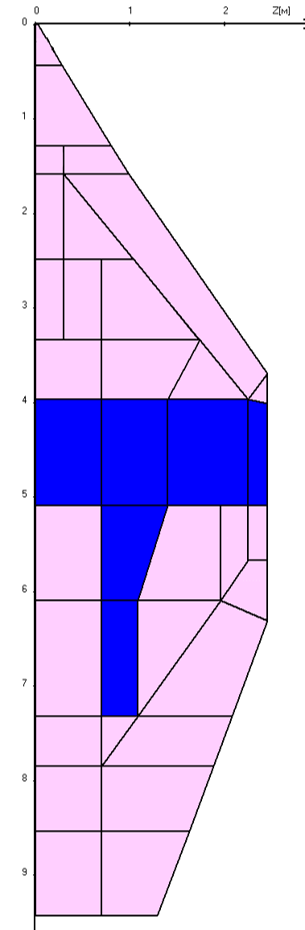
\includegraphics[width=0.3\textwidth]{variants/3_plain}
	\caption{Вариант 3}
\end{subfigure}
\hspace{\fill}
\caption{Схематичные изображения центроплана и соединительной конструкции на виде ``в плане'' половины фюзеляжа }
\label{fig:variants_plain}
\end{figure}	


\begin{figure}[H]
\centering
\begin{subfigure}[b]{0.32\textwidth}
	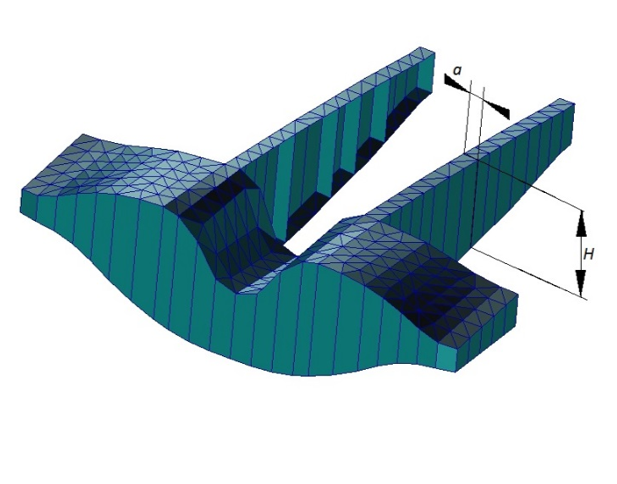
\includegraphics[width=\textwidth]{variants/1_mke}		\caption{Вариант 1}
	\label{fig:variants_mke:1}
\end{subfigure}
\hspace{\fill}
\begin{subfigure}[b]{0.32\textwidth}
	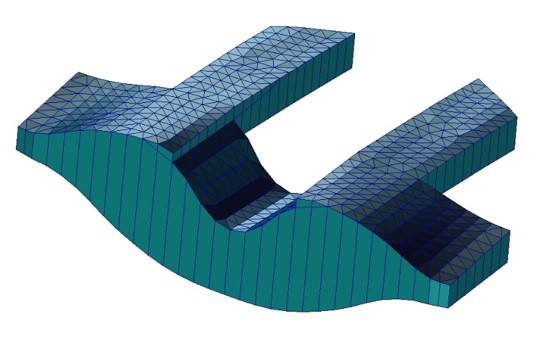
\includegraphics[width=\textwidth]{variants/2_mke}
		\caption{Вариант 2}
		\label{fig:variants_mke:2}
\end{subfigure}
\hspace{\fill}
\begin{subfigure}[b]{0.32\textwidth}
	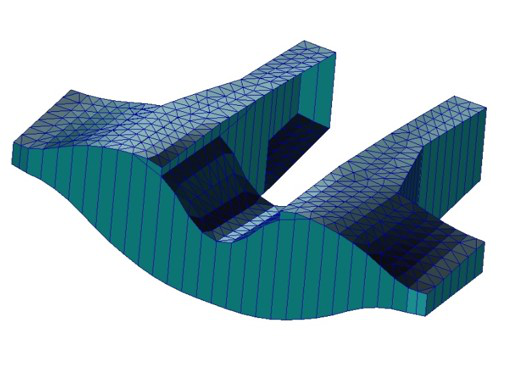
\includegraphics[width=\textwidth]{variants/3_mke}
		\caption{Вариант 3}
		\label{fig:variants_mke:3}
\end{subfigure}
\hspace{\fill}
\caption{Виды МКЭ-моделей центроплана и соединительного элемента}
\label{fig:variants_mke}
\end{figure}	



\section{Подбор оптимальной дискретности модели}
\label{sec:optimalMKESize}

В целях обеспечения точности расчета было проведено исследование зависимости 
НДС гипотетической модели БПЛА, представленной в разделе \ref{sec:creationOfOneModel} (именуемой далее базовой моделью), от максимального характерного размера конечных элементов, используемых в модели. 

С помощью программного комплекса ``Conver'' на основе базовой модели было построено 7 моделей БПЛА, отличающихся лишь максимальным размером конечных элементов, используемых при построении модели. Для сравнительного анализа моделей были выбраны четыре точки, в которых, в соответствии с результатами, полученными в разделе \ref{sec:ndsResults}, обнаруживаются наибольшие напряжения. Путем расчета полученных моделей с помощью программного продукта MSC.Nastran были получены величины напряжений в этих четырех точках для каждой модели.

%Нужно пересчитывать график

\begin{figure}[ht]
\centering
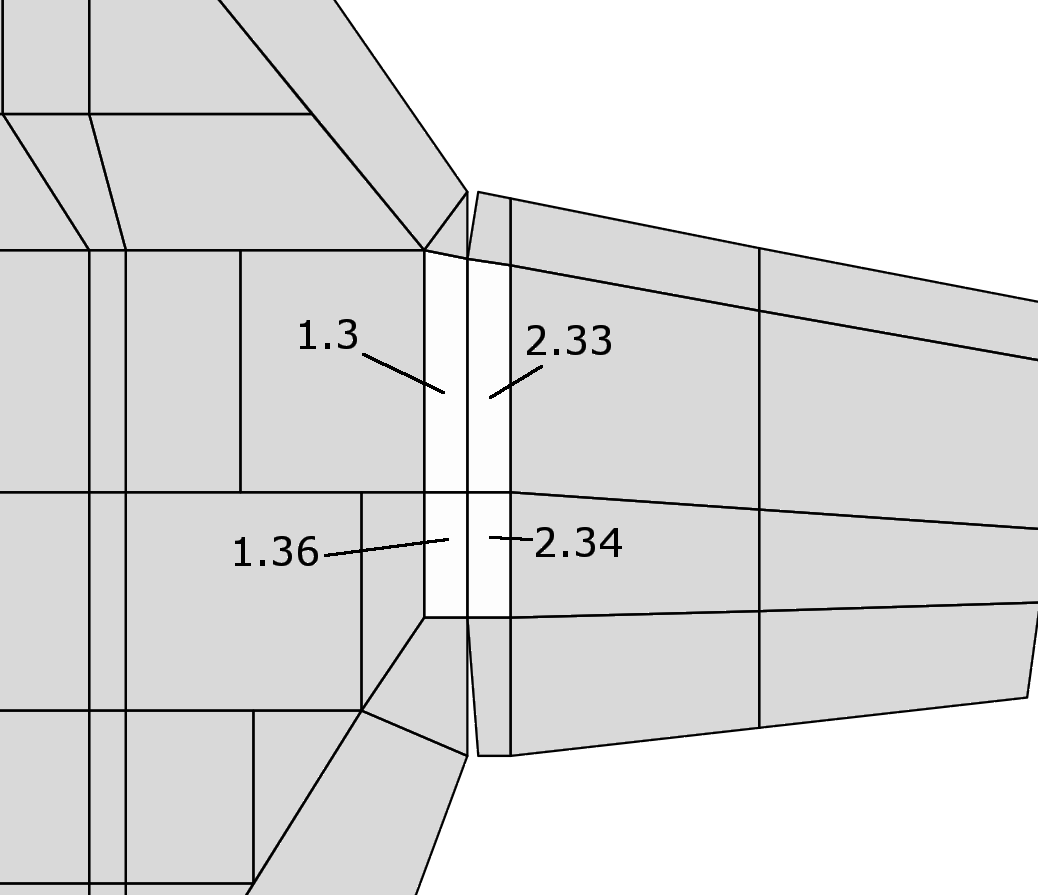
\includegraphics[width=0.5\textwidth]{RootOfWingWithSelectedPartsBW}
\caption{Схематичное изображение вида сверху в месте стыка правого крыла и фюзеляжа}
\label{fig:WingRootPlain}
\end{figure}


\begin{figure}[H]
\captionsetup{justification=centering}
\centering
	\begin{subfigure}[b]{0.8\textwidth}
	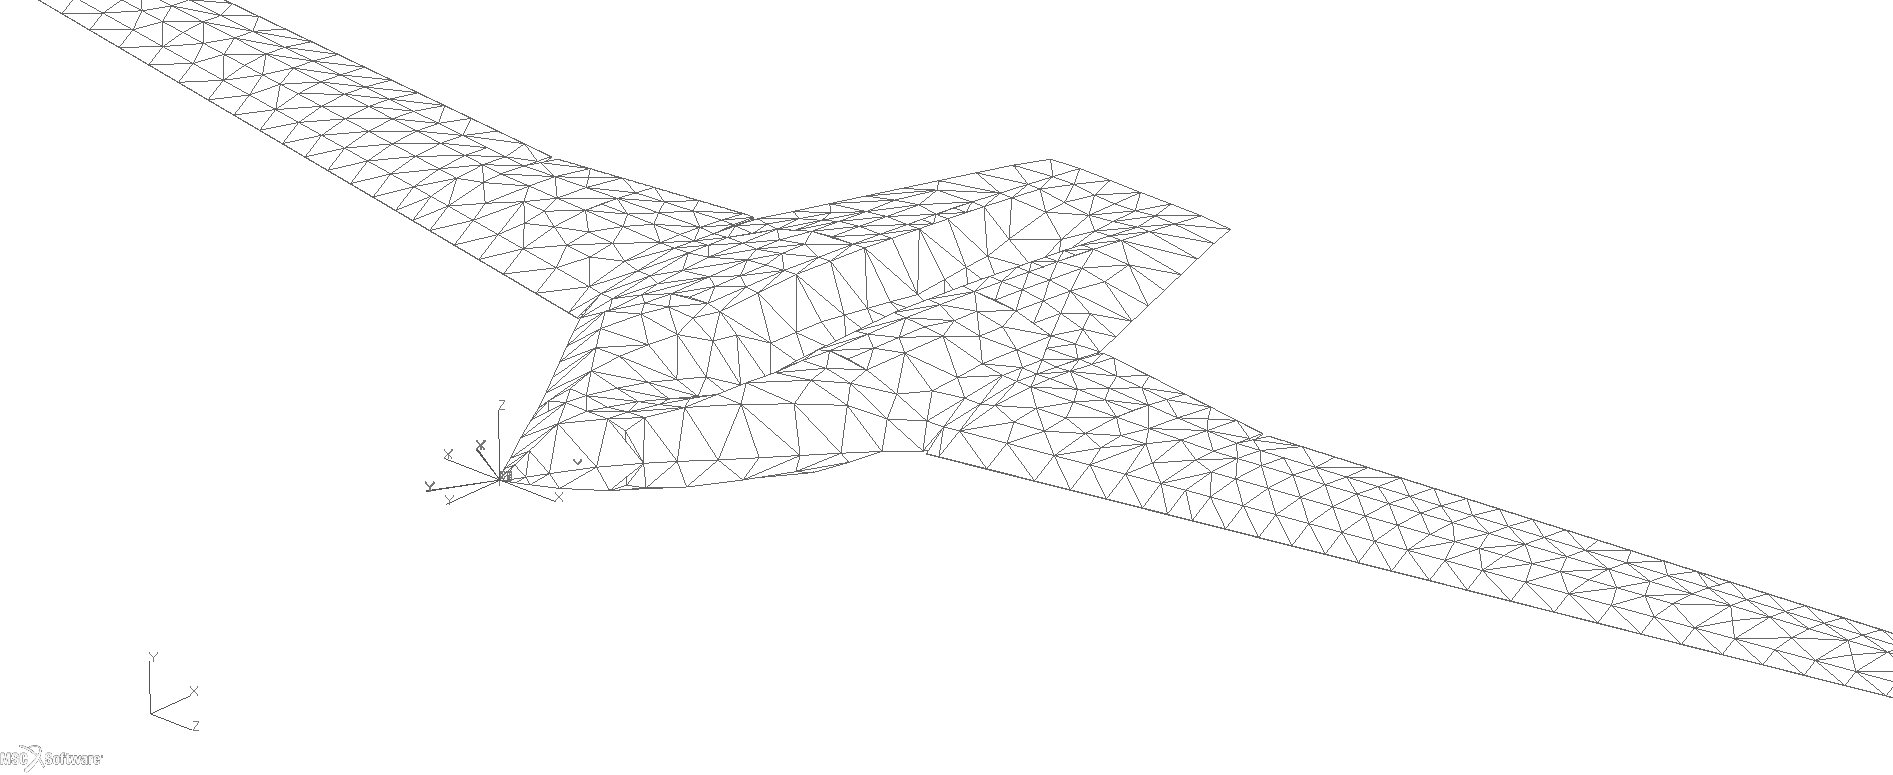
\includegraphics[width=0.98\textwidth]{discreteness/0_4}
	\caption{$L_\text{КЭ} = 0.4см$}
	\label{fig:discr:0_4}
	\end{subfigure}
	\begin{subfigure}[b]{0.8\textwidth}
	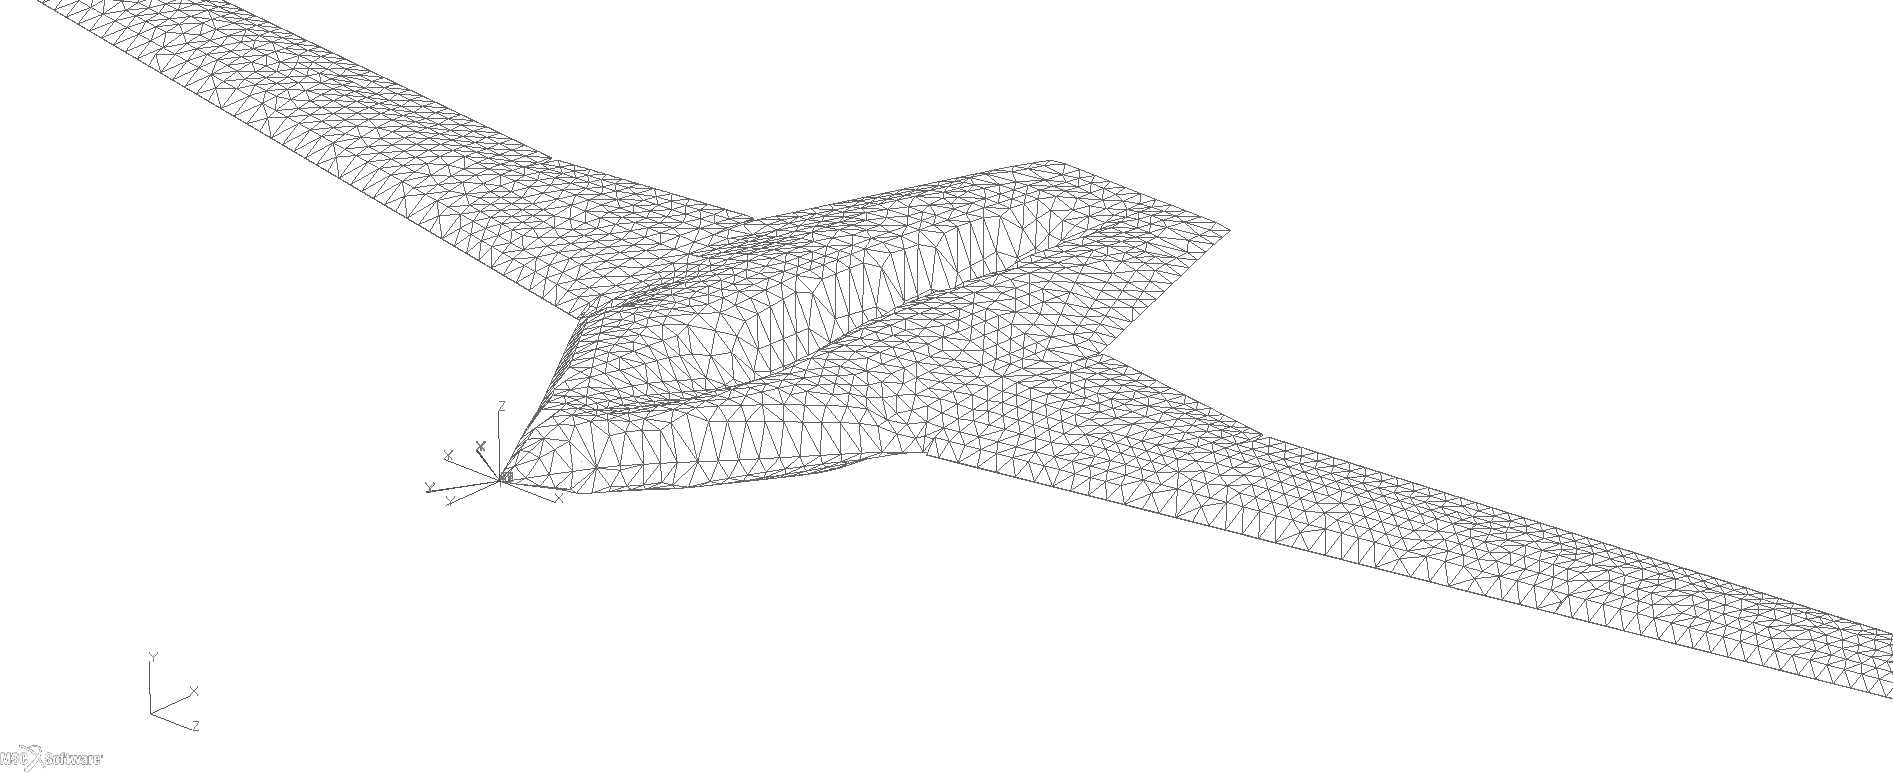
\includegraphics[width=0.98\textwidth]{discreteness/0_2}
	\caption{$L_\text{КЭ} = 0.2см$}
	\label{fig:discr:0_2}
	\end{subfigure}
	\begin{subfigure}[b]{0.8\textwidth}
	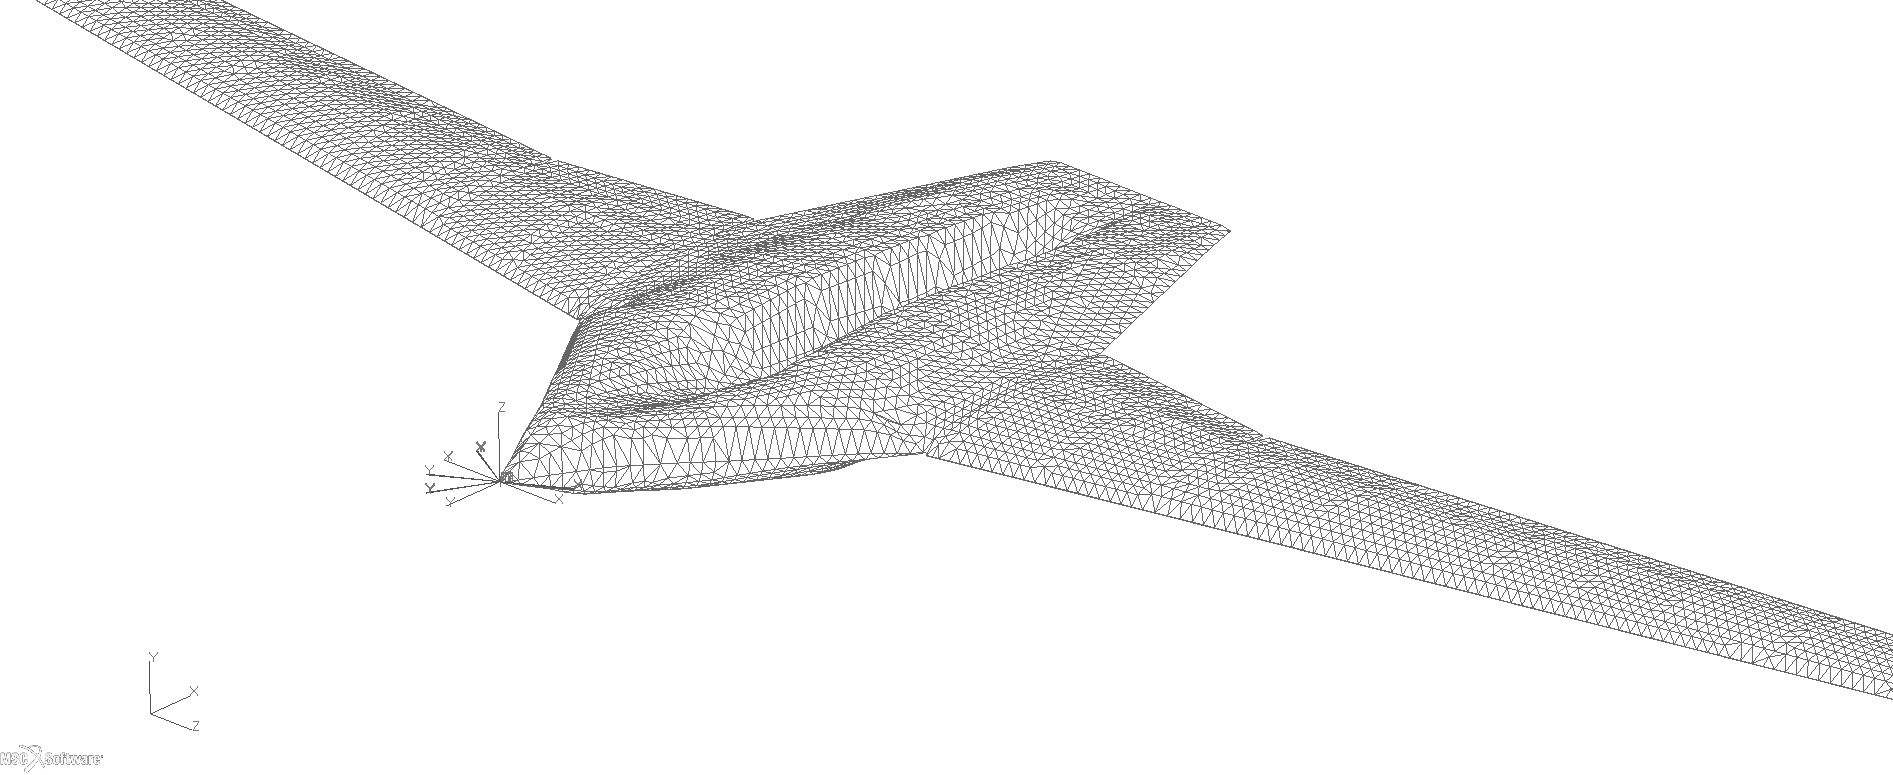
\includegraphics[width=0.98\textwidth]{discreteness/0_13}
	\caption{$L_\text{КЭ} = 0.13см$}
	\label{fig:discr:0_13}
	\end{subfigure}
\label{fig:discreteness}
\caption{Изображения МКЭ-моделей гипотетического БПЛА, построенных с использованием различных характерных размеров конечного элемента}
\end{figure}



На Рис.\ref{fig:stressToDiscreteness} представлена зависимость найденых эквивалентных напряжений (напряжений по Мизесу) в выбранных точках от максимального размера конечного элемента, используемого при построении модели. 

\begin{figure}[H]
\centering
%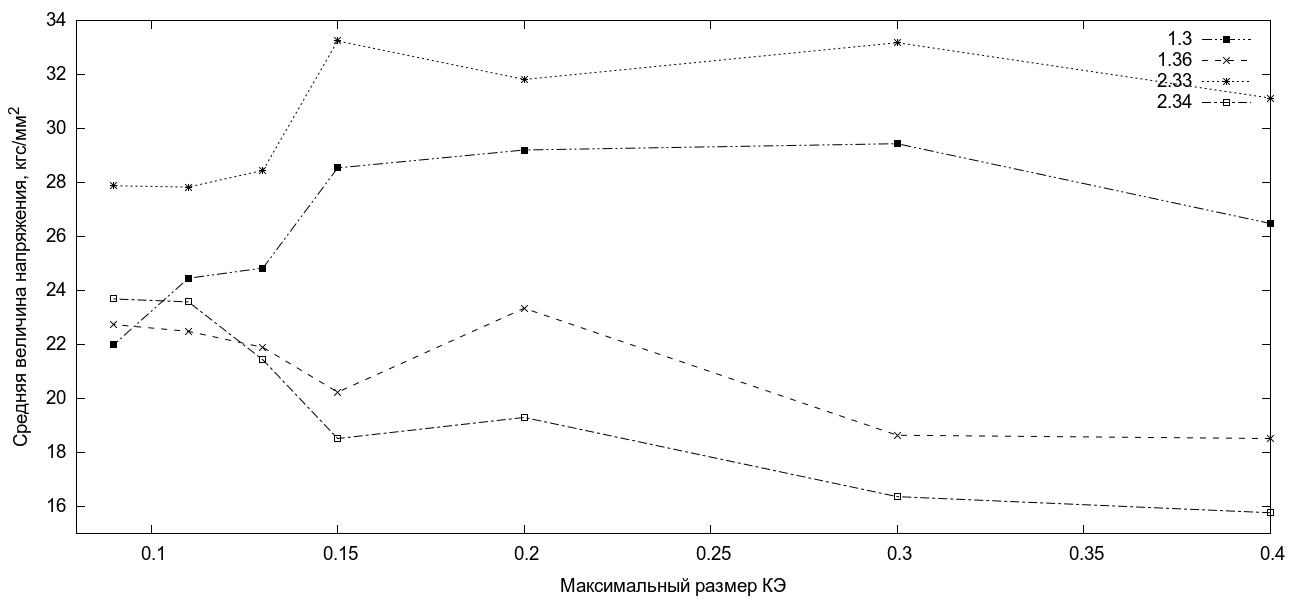
\includegraphics[width=0.8\textwidth]{StressToDiscretenessPlot}
\def\svgwidth{\textwidth}
% GNUPLOT: LaTeX picture with Postscript
\begingroup
  \makeatletter
  \providecommand\color[2][]{%
    \GenericError{(gnuplot) \space\space\space\@spaces}{%
      Package color not loaded in conjunction with
      terminal option `colourtext'%
    }{See the gnuplot documentation for explanation.%
    }{Either use 'blacktext' in gnuplot or load the package
      color.sty in LaTeX.}%
    \renewcommand\color[2][]{}%
  }%
  \providecommand\includegraphics[2][]{%
    \GenericError{(gnuplot) \space\space\space\@spaces}{%
      Package graphicx or graphics not loaded%
    }{See the gnuplot documentation for explanation.%
    }{The gnuplot epslatex terminal needs graphicx.sty or graphics.sty.}%
    \renewcommand\includegraphics[2][]{}%
  }%
  \providecommand\rotatebox[2]{#2}%
  \@ifundefined{ifGPcolor}{%
    \newif\ifGPcolor
    \GPcolorfalse
  }{}%
  \@ifundefined{ifGPblacktext}{%
    \newif\ifGPblacktext
    \GPblacktexttrue
  }{}%
  % define a \g@addto@macro without @ in the name:
  \let\gplgaddtomacro\g@addto@macro
  % define empty templates for all commands taking text:
  \gdef\gplbacktext{}%
  \gdef\gplfronttext{}%
  \makeatother
  \ifGPblacktext
    % no textcolor at all
    \def\colorrgb#1{}%
    \def\colorgray#1{}%
  \else
    % gray or color?
    \ifGPcolor
      \def\colorrgb#1{\color[rgb]{#1}}%
      \def\colorgray#1{\color[gray]{#1}}%
      \expandafter\def\csname LTw\endcsname{\color{white}}%
      \expandafter\def\csname LTb\endcsname{\color{black}}%
      \expandafter\def\csname LTa\endcsname{\color{black}}%
      \expandafter\def\csname LT0\endcsname{\color[rgb]{1,0,0}}%
      \expandafter\def\csname LT1\endcsname{\color[rgb]{0,1,0}}%
      \expandafter\def\csname LT2\endcsname{\color[rgb]{0,0,1}}%
      \expandafter\def\csname LT3\endcsname{\color[rgb]{1,0,1}}%
      \expandafter\def\csname LT4\endcsname{\color[rgb]{0,1,1}}%
      \expandafter\def\csname LT5\endcsname{\color[rgb]{1,1,0}}%
      \expandafter\def\csname LT6\endcsname{\color[rgb]{0,0,0}}%
      \expandafter\def\csname LT7\endcsname{\color[rgb]{1,0.3,0}}%
      \expandafter\def\csname LT8\endcsname{\color[rgb]{0.5,0.5,0.5}}%
    \else
      % gray
      \def\colorrgb#1{\color{black}}%
      \def\colorgray#1{\color[gray]{#1}}%
      \expandafter\def\csname LTw\endcsname{\color{white}}%
      \expandafter\def\csname LTb\endcsname{\color{black}}%
      \expandafter\def\csname LTa\endcsname{\color{black}}%
      \expandafter\def\csname LT0\endcsname{\color{black}}%
      \expandafter\def\csname LT1\endcsname{\color{black}}%
      \expandafter\def\csname LT2\endcsname{\color{black}}%
      \expandafter\def\csname LT3\endcsname{\color{black}}%
      \expandafter\def\csname LT4\endcsname{\color{black}}%
      \expandafter\def\csname LT5\endcsname{\color{black}}%
      \expandafter\def\csname LT6\endcsname{\color{black}}%
      \expandafter\def\csname LT7\endcsname{\color{black}}%
      \expandafter\def\csname LT8\endcsname{\color{black}}%
    \fi
  \fi
  \setlength{\unitlength}{0.0500bp}%
  \begin{picture}(8502.00,4534.00)%
    \gplgaddtomacro\gplbacktext{%
      \csname LTb\endcsname%
      \put(814,892){\makebox(0,0)[r]{\strut{} 16}}%
      \put(814,1267){\makebox(0,0)[r]{\strut{} 18}}%
      \put(814,1642){\makebox(0,0)[r]{\strut{} 20}}%
      \put(814,2017){\makebox(0,0)[r]{\strut{} 22}}%
      \put(814,2393){\makebox(0,0)[r]{\strut{} 24}}%
      \put(814,2768){\makebox(0,0)[r]{\strut{} 26}}%
      \put(814,3143){\makebox(0,0)[r]{\strut{} 28}}%
      \put(814,3518){\makebox(0,0)[r]{\strut{} 30}}%
      \put(814,3894){\makebox(0,0)[r]{\strut{} 32}}%
      \put(814,4269){\makebox(0,0)[r]{\strut{} 34}}%
      \put(1393,484){\makebox(0,0){\strut{} 0.1}}%
      \put(2512,484){\makebox(0,0){\strut{} 0.15}}%
      \put(3631,484){\makebox(0,0){\strut{} 0.2}}%
      \put(4749,484){\makebox(0,0){\strut{} 0.25}}%
      \put(5868,484){\makebox(0,0){\strut{} 0.3}}%
      \put(6986,484){\makebox(0,0){\strut{} 0.35}}%
      \put(8105,484){\makebox(0,0){\strut{} 0.4}}%
      \put(176,2486){\rotatebox{-270}{\makebox(0,0){\strut{}Средняя величина напряжения, $\text{кгс}/\text{мм}^2$}}}%
      \put(4525,154){\makebox(0,0){\strut{}Максимальный размер КЭ}}%
    }%
    \gplgaddtomacro\gplfronttext{%
      \csname LTb\endcsname%
      \put(7118,4096){\makebox(0,0)[r]{\strut{}$1.3$}}%
      \csname LTb\endcsname%
      \put(7118,3876){\makebox(0,0)[r]{\strut{}$1.36$}}%
      \csname LTb\endcsname%
      \put(7118,3656){\makebox(0,0)[r]{\strut{}$2.33$}}%
      \csname LTb\endcsname%
      \put(7118,3436){\makebox(0,0)[r]{\strut{}$2.34$}}%
    }%
    \gplbacktext
    \put(0,0){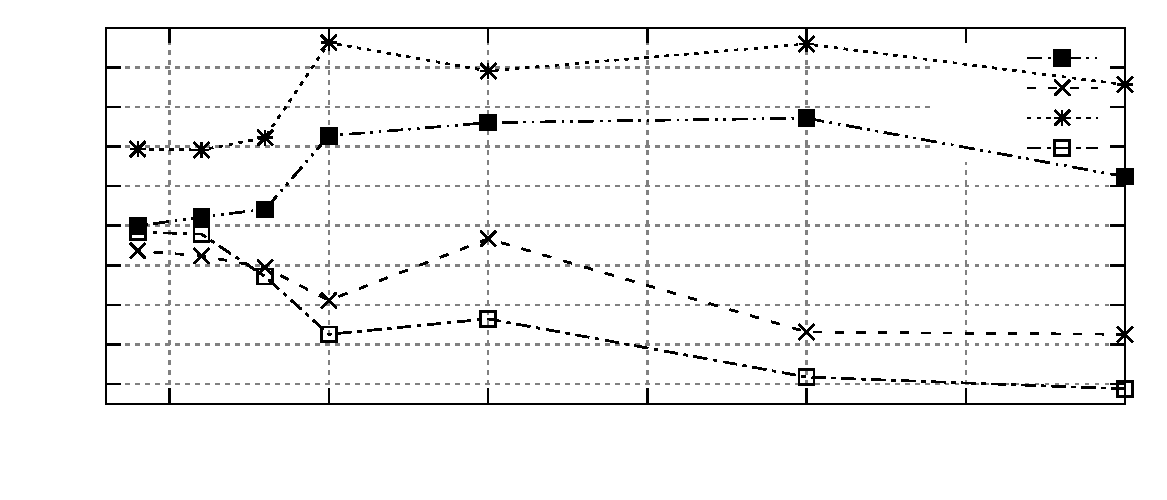
\includegraphics{StressToDiscreteness}}%
    \gplfronttext
  \end{picture}%
\endgroup

\caption{Зависимость напряжений в выбранных точках от максимальной величины КЭ, используемой в модели}
\label{fig:stressToDiscreteness}
\end{figure}


	

Исходя из полученных данных и с учетом зависимости трудоемкости процесса от максимального размера КЭ, была определена оптимальная для дальнейших параметрических исследований моделей гипотетического БПЛА величина конечного элемента, равная $0,11\text{м}$. 
%Ниже приведены картины НДС в месте стыка крыла с фюзеляжем при различных размерах конечного элемента. 


\section{Сравнение моделей}

Как было описано выше, в работе был проведен сравнительный анализ трех вариантов конструкции элемента, обеспечивающего крепление хвостовой части фюзеляжа к центроплану. Первый вариант представляет собой длинный узкий короб с несколькими перегородками (Рис.\ref{fig:variants_mke:1}). В первом варианте двигатель крепится в двух местах непосредственно к стенке короба. Данный вариант частично соответствует модельному варианту n стенок с $n = 4$, рассмотренному в разделе \ref{sec:pants}. Во втором варианте используется широкий плоский короб, частично расположенный над шассийной нишей (Рис.\ref{fig:variants_mke:2}). В данном варианте двигатель крепится к стенке короба и на боковое ребро короба. Третий вариант является промежуточным между первым и вторым и представляет собой широкий короб, соответствующий по высоте фюзеляжной части центроплана в месте их крепления (Рис.\ref{fig:variants_mke:3}). В данном варианте двигатель крепится аналогично второму варианту. 

В ходе сравнительного анализа моделей был проведен МКЭ-расчет созданных моделей с помощью программного продукта MSC.Nastran. В результате расчета были получены напряженно-деформированные состояния каждой из моделей. Ниже приведено сравнение весовых характеристик моделей. Нумерация моделей в таблице соответствует нумерации на рисунках \ref{fig:variants_plain} и \ref{fig:variants_mke}

\tabulinesep = 1mm
\definecolor{lightgray}{gray}{0.9}
\begin{table}[H]
\captionsetup{justification=centering}
\caption{Таблица весовых характеристик моделей}
\begin{tabu}to \linewidth{*4{|X[m c]}|}
\hline
\taburowcolors {lightgray .. white}
 & Вариант 1 & Вариант 2 & Вариант 3 \\ \hline
масса фюзеляжа & 850кг & 812кг  & 778кг \\ \hline
относительная масса фюзеляжа & $100\%$ & $95\%$ & $91,5\%$ \\ \hline
%масса обшивки & 489кг & 505кг  & 499кг \\ \hline
%масса подкрепляющего набора & 361кг & 307кг  & 277кг \\ \hline
\end{tabu}
\label{tab:variantsMasses}
\end{table}

Из полученных данных сделан вывод о том, что оптимальным по весовым характеристикам является использование третьего варианта конструкции. 

